\documentclass[12pt]{report}

\usepackage{graphicx}
\usepackage{float}
%\usepackage{biblatex}
\usepackage[a4paper, margin=1in]{geometry}
\usepackage[backend=biber,style=numeric]{biblatex}
\addbibresource{references.bib}
\usepackage{url}  % for clickable URLs in bibliography


\makeatletter
\renewcommand{\maketitle}{
\begin{center}

\pagestyle{empty}
\phantom{.}  %necessary to add space on top before the title
\vspace{0.5cm}

{\Huge \bf \@title\par}
\vspace{5cm}

{\LARGE Zülal Uludoğan, 2444057}\\[0.5cm]
{\LARGE Ahmet Taha Çelik, 2515831}

\vfill

{\Large\@date}

\end{center}
}\makeatother
\begin{document}
\begin{center}
    \hspace{0.5cm}
\includegraphics[scale=1.2]{figures/metu_eelogo.png}
\end{center}

\title{Middle East Technical University \\[0.5cm]
EE446 Computer Architecture II \\[0.5cm]
Term Project Report}

\author{Ahmet Taha Çelik, Zülal Uludoğan}
\date{25 May 2025}

\maketitle
\tableofcontents

\chapter{Introduction}

\section{Project Description}

\paragraph{}
This project involves the implementation of a single-cycle RISC-V processor using Verilog HDL, supporting core RV32I instructions such as arithmetic, logic, load/store, and control flow operations. The processor is built in a modular way, with separate units for the datapath, controller, register file, memory, ALU, and UART. The list of supported instructions is shown in Table~\ref{tab:instr_list}. See \cite{harris2021}  and \cite{riscv_spec2024} more details.

\vspace{-3em}
\begin{table}[h]
    \centering
    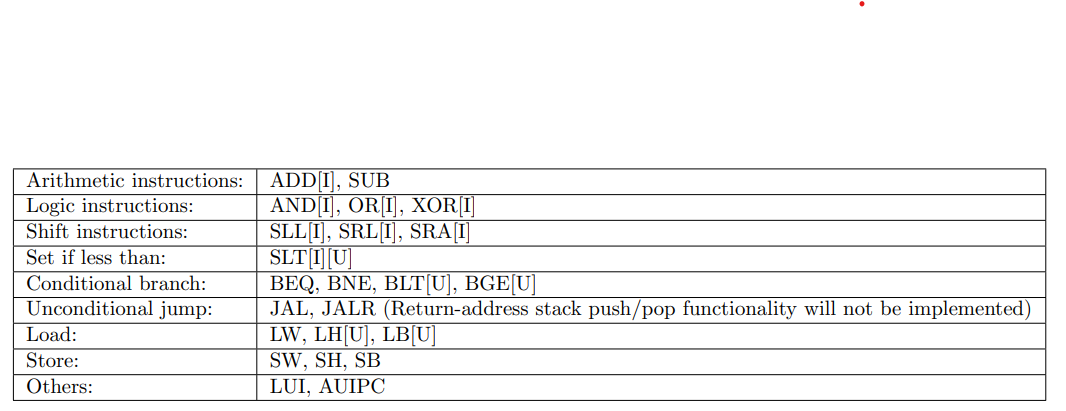
\includegraphics[width=0.8\textwidth]{figures/instr_list.png}
    \caption{List of Instructions}
    \label{tab:instr_list}
\end{table}
\vspace{-1em}

\paragraph{}
The design focuses on correct instruction decoding, datapath control, and memory-mapped I/O integration. The UART module enables serial communication by assigning specific load/store instructions to dedicated addresses, and handles synchronization between different clock domains using FIFO buffers.

\paragraph{}
For verification, a Python-based performance model of the processor is developed and simulated using Cocotb. This model checks instruction behavior cycle-by-cycle and compares the internal states of the Verilog DUT with the expected results, allowing precise debugging and validation of processor functionality. The project demonstrates key concepts in RISC-V architecture, digital system design, and hardware verification through software-driven simulation.





\chapter{Datapath Module}
\begin{figure}[h]
    \centering
    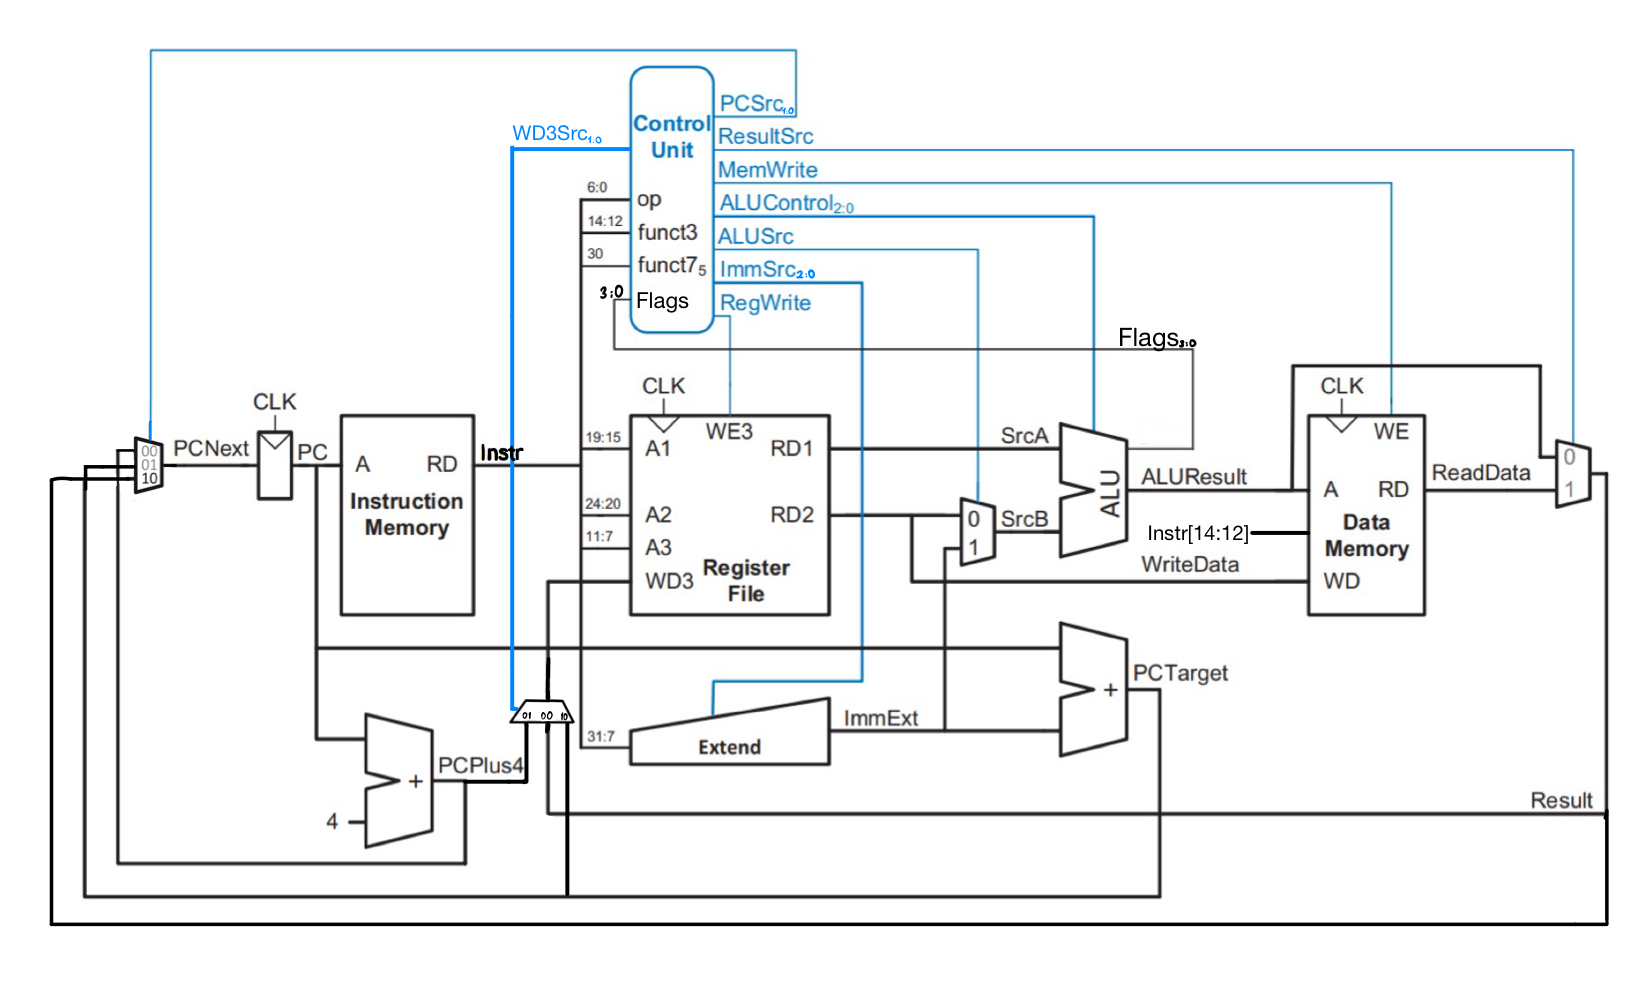
\includegraphics[width=\textwidth]{figures/datapath_flow.jpeg}
    \caption{Modified RISC-V Single Cycle Computer}
    \label{fig:datapath}
\end{figure}

\paragraph{}
The datapath module is responsible for executing instructions defined in the RISC-V ISA, supporting the instruction types listed in Table~\ref{tab:instr_list}. Most submodules were adapted from laboratory components, but modifications were made to support specific instruction semantics and to align with the RISC-V architecture. A synchronous reset (\texttt{RESET}) is integrated into the module to ensure all registers and memory components are properly initialized.

\paragraph{}
Unlike ARM, where 16 general-purpose registers are used, the RISC-V register file consists of 32 registers. Register \texttt{x0} is hardwired to zero, as per the RISC-V specification. A 5-to-32 decoder and a 32-to-1 multiplexer are used to handle register selection and writing. The \texttt{Register\_file} module supports debug output and dual read ports, along with a single write port controlled by the \texttt{RegWrite} signal.

\begin{figure}[h]
    \centering
    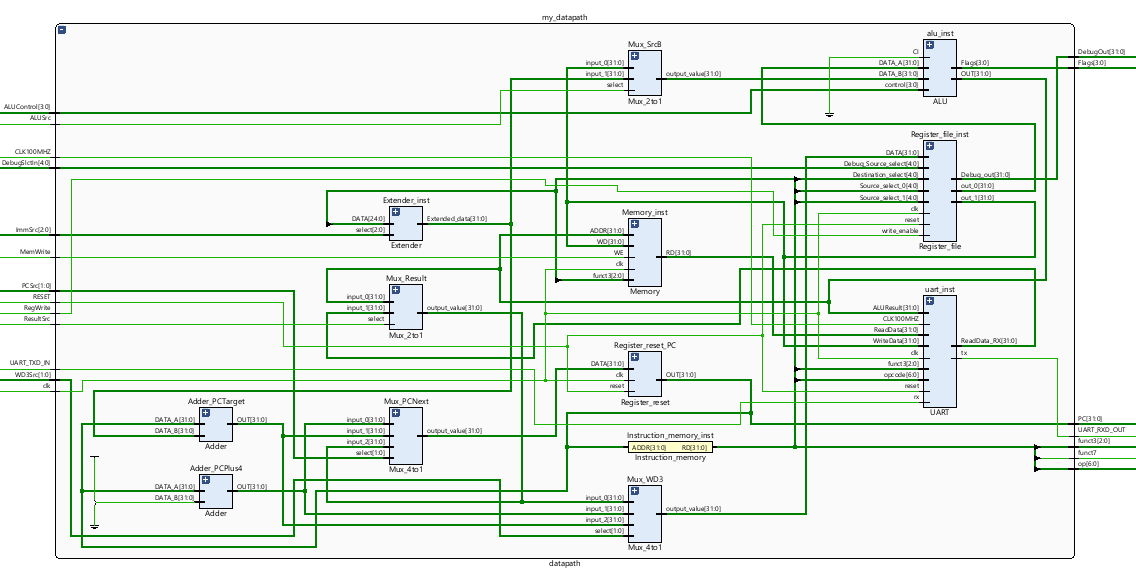
\includegraphics[width=\textwidth]{figures/rtl_datapath.png}
    \caption{Synthesized RTL view of the datapath module}
    \label{fig:datapath_rtl}
\end{figure}

\paragraph{}
The datapath is designed to handle all six RISC-V instruction types—R-type, I-type, S-type, B-type, U-type, and J-type—by routing operands and control signals through shared hardware blocks and dedicated control logic. Each instruction type makes use of a subset of datapath components to perform its operation.

\paragraph{R-type Instructions}
R-type instructions perform register-to-register arithmetic and logical operations. The instruction provides two source registers (\texttt{rs1} and \texttt{rs2}) and a destination register (\texttt{rd}). The values from \texttt{rs1} and \texttt{rs2} are read from the register file and passed to the ALU. The ALU performs the operation specified by the \texttt{funct3} and \texttt{funct7} fields (e.g., \texttt{ADD}, \texttt{SUB}, \texttt{SLL}), and the result is written back to \texttt{rd} through the \texttt{WD3} multiplexer.

\paragraph{I-type Instructions}
I-type instructions include immediate arithmetic/logical operations (e.g., \texttt{ADDI}, \texttt{ANDI}), loads (e.g., \texttt{LW}, \texttt{LB}), and \texttt{JALR}. These instructions use one source register and an immediate. The immediate is sign-extended by the \texttt{Extender} module, then used as an operand in the ALU or as an offset for memory access. For arithmetic instructions, the ALU result is written back to \texttt{rd}. For load instructions, the data is read from memory and passed through the \texttt{Result} multiplexer to be written to the register file.

\paragraph{S-type Instructions}
S-type instructions are store instructions such as \texttt{SW}, \texttt{SH}, and \texttt{SB}. These use two source registers: \texttt{rs1} provides the base address, and \texttt{rs2} provides the data to be stored. The immediate is generated by concatenating two fields and sign-extended. The memory address is computed by adding the immediate to \texttt{rs1}, and the result is used by the memory module to perform the store.

\paragraph{B-type Instructions}
B-type instructions are conditional branches such as \texttt{BEQ}, \texttt{BNE}, and \texttt{BLT}. The two source registers are compared using the ALU, which performs subtraction and sets condition flags. If the branch condition is met, the program counter is updated to \texttt{PC + immediate}; otherwise, it proceeds sequentially. The \texttt{PCSrc} signal controls which address is selected via the \texttt{PCNext} multiplexer.

\paragraph{U-type Instructions}
U-type instructions such as \texttt{LUI} and \texttt{AUIPC} use a 20-bit immediate value shifted left by 12 bits. For \texttt{LUI}, the immediate is written directly into the destination register. For \texttt{AUIPC}, the immediate is added to the current PC and the result is written back to \texttt{rd}. The extended immediate is generated by the \texttt{Extender} and routed through the \texttt{Mux\_WD3} path.

\paragraph{J-type Instructions}
J-type instructions, specifically \texttt{JAL}, perform an unconditional jump to a target address calculated from the PC and a 21-bit immediate. Before jumping, the return address (\texttt{PC + 4}) is saved into \texttt{rd}. The PC update logic and the \texttt{Mux\_WD3} handle this behavior, and the control signals ensure the correct values are selected and stored.

\paragraph{}
Each instruction type is supported through coordinated control of multiplexers, the ALU, the register file, the extender, and memory modules, all synchronized by the controller to ensure correct execution paths across the datapath.


\begin{figure}[h]
    \centering
    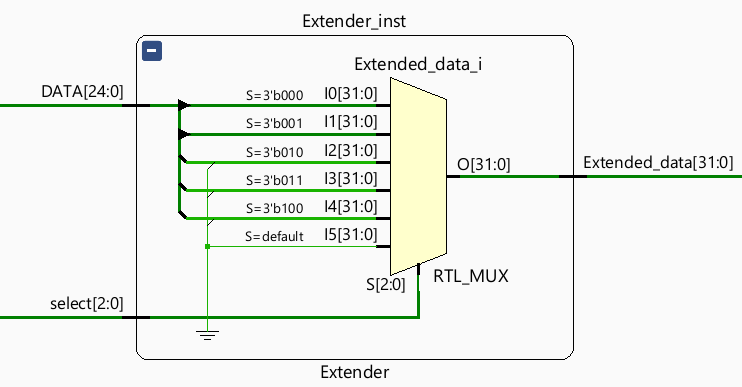
\includegraphics[width=0.8\textwidth]{figures/rtl_extender.png}
    \caption{Synthesized RTL view of the extender module}
    \label{fig:extender rtl}
\end{figure}

\paragraph{}
All arithmetic and logic operations, including shift operations, are implemented inside the \texttt{ALU} module. Shift instructions use immediate values or register contents as shift amounts, and the ALU supports logical (\texttt{SRL}) and arithmetic (\texttt{SRA}) shifts accordingly. For branch instructions such as \texttt{BEQ} and \texttt{BNE}, the ALU performs a subtraction to set condition flags, which are later evaluated in the control path to determine branch decisions.

\paragraph{}
The \texttt{Memory} module is adapted to support byte (\texttt{LB}/\texttt{SB}), halfword (\texttt{LH}/\texttt{SH}), and word (\texttt{LW}/\texttt{SW}) memory accesses. It uses the \texttt{funct3} field of the instruction to determine the access width and whether sign-extension or zero-extension should be applied to loaded data. For store operations, it selectively writes the relevant portion (byte/halfword/word) of the register data into memory without modifying adjacent memory locations.


\chapter{Controller Module}

\paragraph{}
The controller module is responsible for generating the control signals necessary to guide the datapath during the execution of RISC-V instructions. As shown in Figure \ref{fig:controller}, the controller design follows a modular approach and includes three functional units: the \texttt{MainDecoder}, the \texttt{ALUDecoder}, and the \texttt{PCLogic} unit.

\begin{figure}[h]
    \centering
    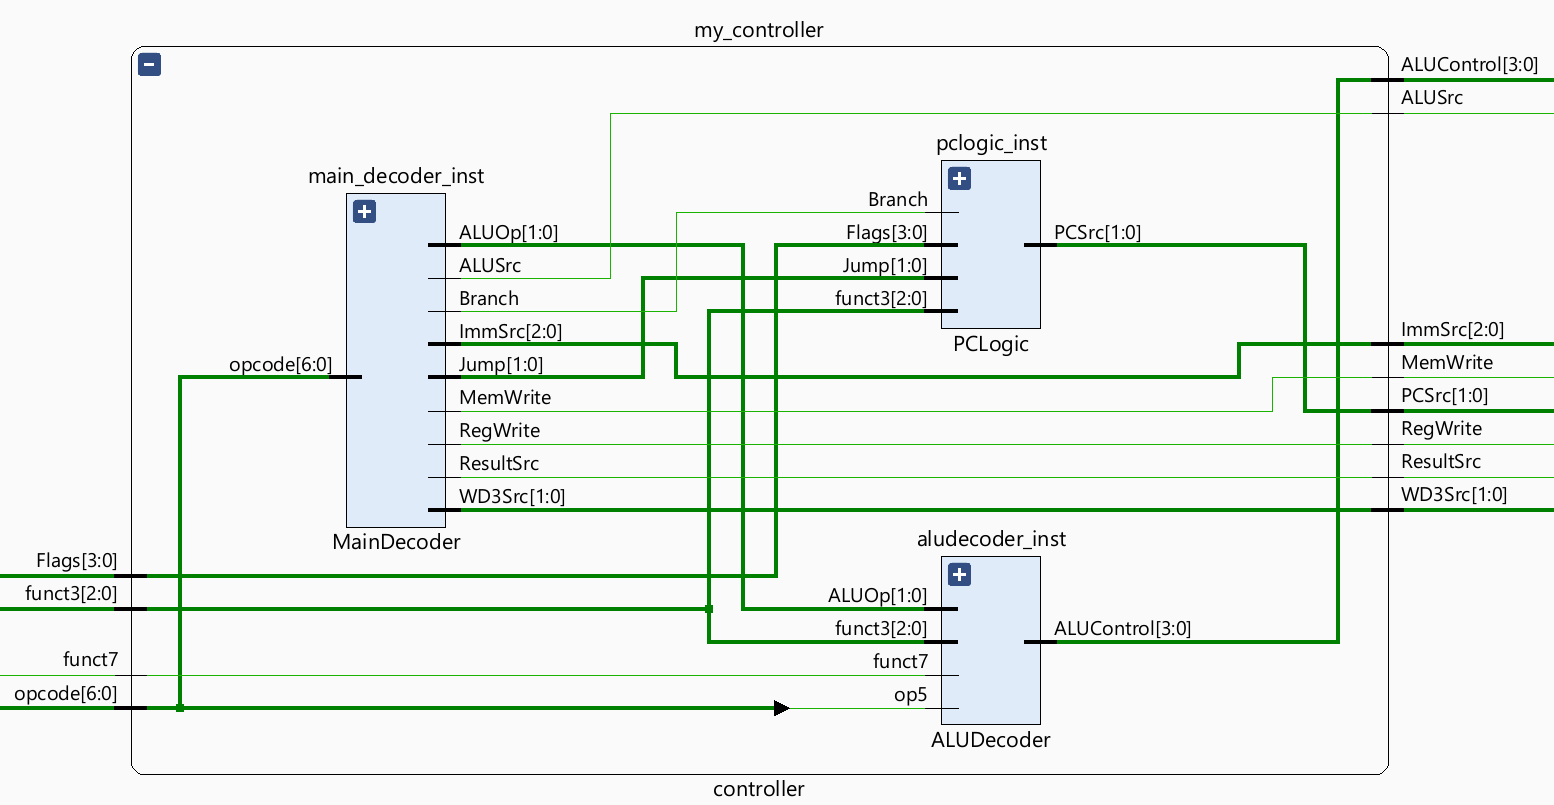
\includegraphics[width=\textwidth]{figures/controller_rtl.png}
    \caption{Synthesized RTL view of the controller module}
    \label{fig:controller}
\end{figure}

\paragraph{}
The \texttt{MainDecoder} interprets the 7-bit opcode from the instruction and produces the primary control signals required by the datapath, such as register file write enable, memory write enable, ALU source selection, and immediate format selection. These signals are then distributed to the corresponding components to orchestrate the processor's behavior.

\paragraph{}
The \texttt{ALUDecoder} further refines control signal generation by examining the \texttt{funct3}, \texttt{funct7}, and other opcode-specific bits to determine the specific ALU operation to perform. It outputs a 4-bit \texttt{ALUControl} signal, ensuring the correct arithmetic or logical operation is selected based on the instruction type.

\paragraph{}
The \texttt{PCLogic} unit handles program counter selection. It considers both the branching conditions and the jump instructions to compute the correct value of the \texttt{PCSrc} signal. This logic is critical for implementing both conditional and unconditional control-flow changes in the processor.

\paragraph{}
The modularity of this controller design simplifies debugging and testing. Each submodule is implemented independently and tested in isolation before integration into the main controller unit.


\chapter{UART Module}

\paragraph{}
The UART (Universal Asynchronous Receiver-Transmitter) module is responsible for facilitating serial communication between the RISC-V processor and external systems. Its implementation involved significantly more complexity than the controller module due to the nature of asynchronous communication, timing constraints, and the need to bridge two separate clock domains. Figure \ref{fig:uart} shows the synthesized RTL view of the UART subsystem.

\begin{figure}[h]
    \centering
    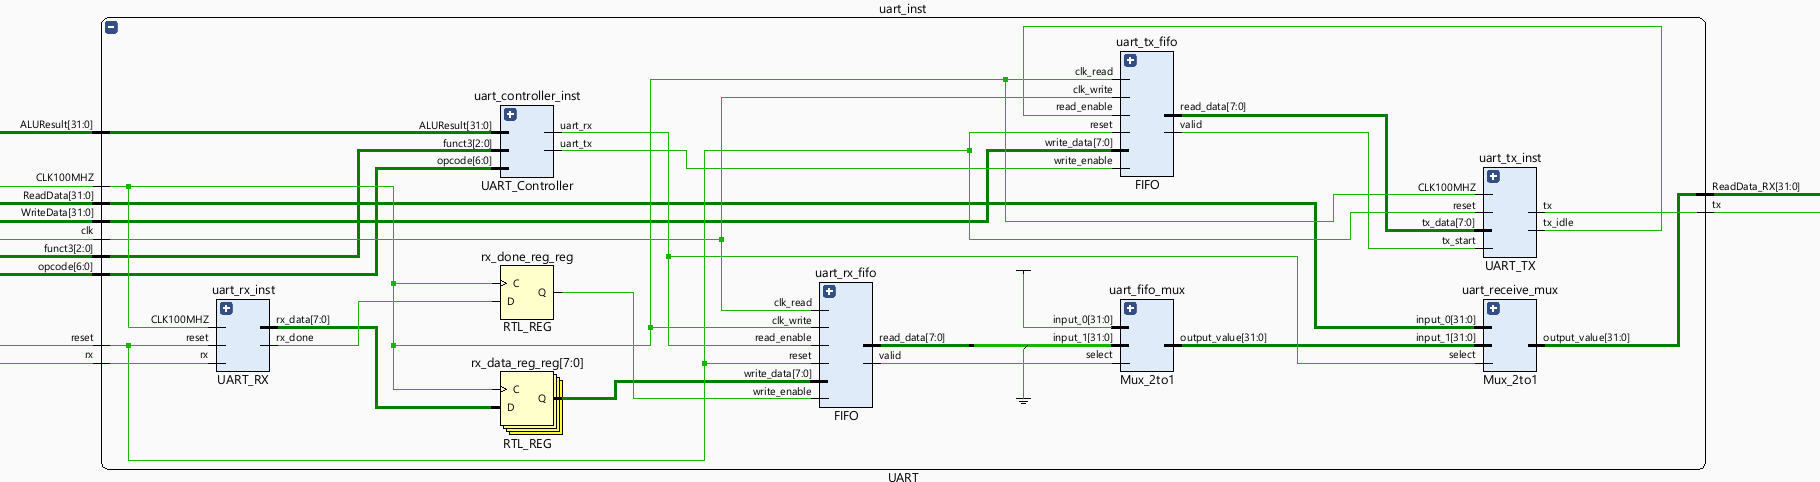
\includegraphics[width=\textwidth]{figures/uart_rtl.png}
    \caption{Synthesized RTL view of the UART module}
    \label{fig:uart}
\end{figure}

\section{Design Overview}

\paragraph{}
The UART module integrates both transmitting and receiving functionalities while adhering to the 9600 baud 8-N-1 protocol. Memory-mapped I/O is used to send and receive bytes via store and load instructions to addresses \texttt{0x400} and \texttt{0x404}, respectively. When a store is made to \texttt{0x400}, a byte is written to the transmitter FIFO and scheduled for transmission. When a load is performed from \texttt{0x404}, the system reads the most recent byte from the receive FIFO; if no byte is available, the value \texttt{0xFFFFFFFF} is returned.

\paragraph{}
The UART controller examines the current instruction's opcode, \texttt{funct3}, and ALU result to determine whether a UART send or receive should be triggered. This controller outputs \texttt{uart\_tx} or \texttt{uart\_rx} flags accordingly.

\section{Clock Domain Challenges and FIFO Synchronization}

\paragraph{}
One of the key challenges in designing the UART module was handling the presence of two independent clocks: a 100 MHz clock (\texttt{CLK100MHZ}) used for UART timing, and a slower user-controlled system clock (\texttt{clk}) used by the processor core and instruction sequencing. These clocks operate asynchronously, making it unsafe to directly transfer data across domains without proper synchronization.

\paragraph{}
To address this, the design uses dual-clock FIFO buffers for UART transmission and reception, each operating with distinct read and write clocks. Specifically, the \texttt{rx\_fifo} writes incoming bytes using \texttt{CLK100MHZ}, since it is fed by the UART receiver module, which samples serial input at high speed. Its read operations are driven by the processor's \texttt{clk}, as the register file reads received data at the system clock rate. Conversely, the \texttt{tx\_fifo} receives data from the processor via \texttt{clk} during store operations to address \texttt{0x400}, and its contents are transmitted by the UART transmitter at \texttt{CLK100MHZ}. 

\paragraph{}
This deliberate separation ensures safe and reliable data movement between asynchronous domains. Without this dual-clock setup, writing data from one domain and reading it from another could cause metastability or timing hazards, potentially corrupting the data. By isolating read and write logic through clock-specific ports in each FIFO, the design maintains correctness and stability throughout UART communication.


\section{UART Transmitter and Receiver}

\paragraph{}
The transmitter module initiates data transmission when a byte is enqueued into the FIFO and the line is idle. It serializes the data byte according to UART protocol and asserts the \texttt{tx\_idle} signal once transmission is complete. If the FIFO holds multiple bytes, they are transmitted sequentially without processor intervention.

\paragraph{}
The receiver module continuously samples the input \texttt{rx} line using \texttt{CLK100MHZ}. When a valid start bit is detected, it begins capturing bits until the full byte is received. A \texttt{done} flag is raised once reception is complete. The received byte is then pushed into the 16-byte FIFO buffer, ensuring that no bytes are lost if the processor is not immediately ready to read.

\section{UART Transmitter and Receiver State Machines}

\paragraph{}
Both the UART transmitter and receiver modules are implemented as finite state machines (FSMs) that operate on the 100 MHz clock and comply with the 9600 baud 8-N-1 UART protocol. Their behaviors are structured as sequential state transitions, and the FSM logic ensures the correct serialization and deserialization of data.

\subsection{Transmitter State Machine}

\paragraph{}
The transmitter FSM begins in the \texttt{IDLE} state, where it waits for the \texttt{start} signal to be asserted, indicating that a new byte is ready for transmission. Upon activation, it transitions to the \texttt{START} state and drives the transmission line low to indicate the start bit. After holding the line low for one baud period, the FSM enters the \texttt{DATA} state, during which each of the 8 data bits is shifted out sequentially, least significant bit first.

\paragraph{}
Once all data bits are transmitted, the FSM transitions to the \texttt{STOP} state. It then drives the line high for one baud period to signal the stop bit. After this, the FSM returns to the \texttt{IDLE} state, sets the \texttt{idle} flag to indicate readiness, and awaits the next start signal.

\paragraph{}
This structure ensures that every byte is framed with a start and stop bit as per UART standards, and the \texttt{idle} output allows external logic to determine when the transmitter is available for the next byte.

\subsection{Receiver State Machine}

\paragraph{}
The receiver FSM also begins in an \texttt{IDLE} state, continuously monitoring the input \texttt{rx} line. Upon detecting a falling edge (start bit), it transitions to the \texttt{START} state and waits half a baud period to sample the start bit in the middle for noise immunity.

\paragraph{}
After verifying the start bit, it transitions to the \texttt{DATA} state, where it samples 8 data bits at one baud interval each. These bits are shifted into a register, with the least significant bit arriving first.

\paragraph{}
Following the data bits, the FSM enters the \texttt{STOP} state to sample the stop bit. If the stop bit is valid (logic high), the FSM sets the \texttt{done} flag and updates the \texttt{data\_out} register with the fully received byte. It then returns to the \texttt{IDLE} state to prepare for the next frame.

\paragraph{}
This approach ensures that bytes are received reliably and with proper framing. The \texttt{done} signal is used to indicate reception completion, allowing external logic to push the received byte into a FIFO buffer or register.

\section{Peripheral Interface and Integration Strategy}

\paragraph{}
The UART module is designed to integrate seamlessly with the existing processor datapath, requiring minimal changes to the overall system architecture. It relies entirely on memory-mapped communication, interpreting store and load instructions to specific addresses as UART transmit and receive operations, respectively. This eliminates the need for additional global control signals or structural changes outside the UART module itself.

\paragraph{}
A key feature of the integration is the \texttt{ReadData\_RX} signal, which is an output of the UART module. This signal is dynamically assigned based on whether the currently executed instruction is a UART receive. If the instruction is a regular memory load, \texttt{ReadData\_RX} simply propagates the value from the data memory, making it identical to \texttt{ReadData}. However, if the instruction is a UART receive, the module substitutes the memory output with a value retrieved from the UART receive FIFO, either the latest received byte or a default fallback value if the buffer is empty.

\paragraph{}
This design allows the UART to be embedded into the system with minimal modification to the datapath. Specifically, the only change required is at the result selection stage, where the processor chooses between the ALU result and the output from memory (or UART). Since this behavior is already governed by an existing multiplexer, no additional control logic is needed. This elegant interface enables UART communication to function transparently within the single-cycle RISC-V system while preserving the simplicity and modularity of the original datapath.


\chapter{Cocotb Testbench}
\paragraph{}
The Cocotb testbenches used in the laboratories of this course, originally designed for ARM architectures, were modified to support the RISC-V instruction set by adapting both the instruction decoder and the performance model components of the test framework. These modifications enabled cycle-accurate simulation of a single-cycle RISC-V processor and allowed for automated verification against a Verilog-based DUT (Device Under Test).

\paragraph{}
In the RISC-V architecture, each instruction is composed of standard fields such as \texttt{opcode}, \texttt{rd}, \texttt{funct3}, \texttt{rs1}, \texttt{rs2}, and \texttt{funct7}, which differ from ARM’s encoding structure. To handle this, a Python class was implemented to parse each 32-bit hexadecimal instruction. The instruction is first converted to a binary string, from which the fields are extracted based on bit positions defined by the RISC-V specification. Additionally, depending on the instruction type (I-type, S-type, B-type, U-type, or J-type), the immediate values are sign-extended accordingly. Instruction decoding is performed using conditional logic that checks combinations of \texttt{opcode}, \texttt{funct3}, and \texttt{funct7} to identify the exact operation (e.g., \texttt{ADD}, \texttt{SUB}, \texttt{LW}, \texttt{BEQ}). The instruction memory content used for verification is partially shown in Figure~\ref{fig:instr}. To obtain the hexadecimal-encoded instructions for the testbench, the RISC-V instruction converter tool was used \cite{rvcodecjs}.


\begin{figure}[h]
    \centering
    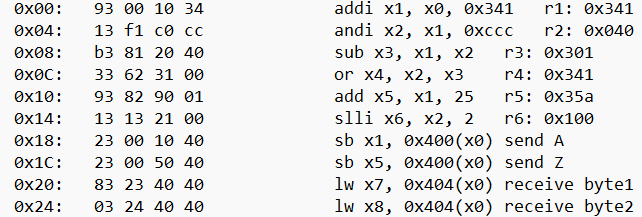
\includegraphics[width=0.6\textwidth]{figures/exp_intrhex.png}
    \caption{Some part of instructions used for the test}
    \label{fig:instr}
\end{figure}

\paragraph{}
To simulate processor behavior, a performance model was developed in Python. This model maintains a register file and a program counter and mimics the functional behavior of the single-cycle processor. A memory abstraction is used to replicate byte-addressable memory and support load and store instructions. The simulation begins by reading instructions from the input file \texttt{Instructions.hex}, reversing their endianness to match the hardware layout, and decoding them using the instruction class. Each instruction is then executed by the performance model, and its effects on the register file and program counter are tracked.

\paragraph{}
At each cycle, the testbench fetches the next instruction, logs its decoding, performs the corresponding operation in the software model, and compares the result with the output of the Verilog design. This includes checking all 32 registers and the PC value. For memory operations, data is either written to or read from the memory abstraction, depending on whether the instruction is a load or store. For control flow instructions such as \texttt{BEQ}, \texttt{BNE}, \texttt{JAL}, and \texttt{JALR}, the program counter is conditionally updated in accordance with the instruction semantics.

 \paragraph{}
In the testbench, UART read operations are simulated by performing a load instruction from the memory-mapped address \texttt{0x00000404}, which corresponds to the UART receive buffer. During normal operation, this address returns the most recently received byte. However, if no data has been received, the UART module is designed to return the default value \texttt{0xFFFFFFFF}. Therefore, within the testbench logic, it is essential to check whether the value read from \texttt{0x00000404} equals \texttt{0xFFFFFFFF}, as this indicates that the receive FIFO is empty and no valid byte is available.

\begin{figure}[h]
    \centering
    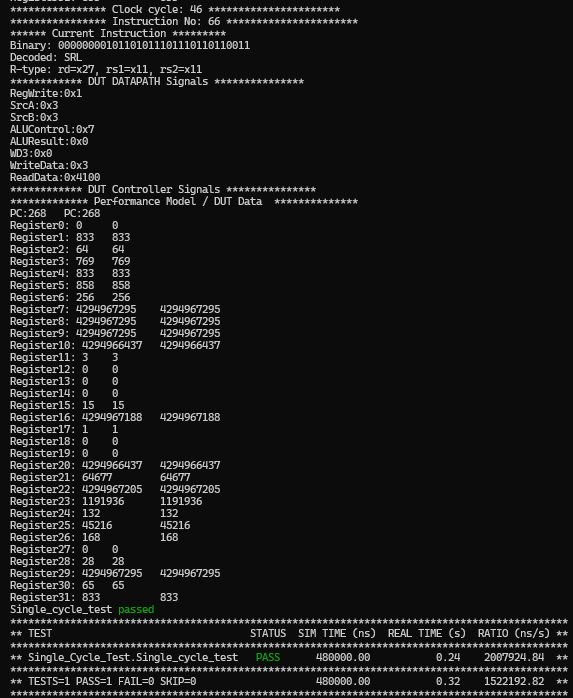
\includegraphics[width=0.6\textwidth]{figures/tb_result.png}
    \caption{An example of testbench result}
    \label{fig:tb result}
\end{figure}

\chapter{Conclusion}

\paragraph{}
In this project, a single-cycle RISC-V processor was successfully designed, implemented, and verified using Verilog HDL and Cocotb. The architecture supports a representative subset of the RV32I instruction set, including arithmetic, logic, memory, and control flow operations. All components—including the datapath, controller, ALU, memory, and UART module—were developed with a modular design philosophy to ensure flexibility and scalability.

\paragraph{}
A key achievement of this work is the integration of a memory-mapped UART module capable of transmitting and receiving data via serial communication. This involved careful management of asynchronous clock domains using dual-clock FIFOs and ensured robust data transfer across the processor and UART interfaces.

\paragraph{}
Verification was accomplished using a custom Python-based performance model and Cocotb testbenches. This approach enabled detailed cycle-by-cycle comparisons between the behavioral model and the Verilog design, helping to identify and resolve functional mismatches during development. The use of Cocotb also facilitated modular testing and improved debugging efficiency.

\paragraph{}
Overall, this project provided hands-on experience with the fundamentals of processor architecture, digital system design, and verification methodologies. Through this work, we gained deeper insights into the RISC-V ISA, HDL-based implementation techniques, and modern verification practices using software-hardware co-simulation.

\printbibliography



\end{document}